\chapter{A survey of justificatory structure}
\label{chap:survey}

Following on from the introduction of various aspects of the justificatory structure of OWL ontologies and interventions for justification encounters in the previous chapters, this chapter presents a survey of the justificatory structure of a set of ontologies from the NCBO BioPortal, a curated collection of over 300 ontologies from the biomedical domain. Given the proposed structure-based coping strategies, we now want to know which structural aspects indeed occur in ontologies used in practice, and to what extent. While we have some knowledge about the occurrence of multiple justifications and some of the structural phenomena found in OWL justifications (e.g. \cite{kalyanpur07oq,horridge11gj,bail11jm}), to date there has been no thorough investigation of the complex relationships between justifications in a large, independently motivated ontology corpus.  

This chapter presents an investigation of the applicability of the theoretical concepts and interventions we have proposed in the previous chapters. The survey presented here indicates the  clinical significance of both the suggested sources of difficulties, as well as the proposed structure-based interventions. In our case, we claim that the significance of phenomenon and intervention corresponds to its \emph{prevalence} in OWL ontologies used in practice: given some OWL ontology, how likely is it for an ontology developer to encounter a source of difficulty, and how likely is it that structure-based coping strategies exist that can be exploited to reduce this difficulty?


%%%%%%%%%%%%


\section{The BioPortal corpus}

In this section, we will describe the properties of the test corpus used in our survey, and outline the justification generation process. The entailment extraction and justification generation comprises several filtering steps, which are motivated by the different types of entailments justifications we have presented in Chapters \ref{chap:entailments} and \ref{chap:structure}: if we simply treated all justifications and entailments equally, regardless of their origin (native, mixed, or imported) or complexity (self-justification, atomic subsumption chain, or complex), we would run risk of over- or understating features of the justificatory structure of the ontologies in our corpus. We therefore filter out entailments---and ontologies---which would skew the justification analysis towards irrelevant types of justifications.


\subsection{Properties of the corpus}

The purpose of this survey is to analyse the justificatory structure of a set of OWL ontologies which is representative for the range of ontologies used in practise. This would exclude tutorial and toy ontologies, such as the well-known \emph{Pizza} and \emph{Koala} ontologies, which were specifically built for the purpose of demonstrating certain OWL features, or might be very small and inexpressive. In order to prevent bias through hand-picking \enquote{suitable} ontologies, our aim was to use an independently motivated corpus of ontologies. Thus, the choice was between a random sample of web ontologies (e.g. obtained from a web crawl) and an existing ontology repository. As the NCBO BioPortal ontology repository contains a large number of actively used and well-studied ontologies which cover a broad spectrum of size and expressivity, it seemed a suitable choice for an extensive survey of justificatory structure. 

BioPortal is a web-based ontology repository which provides over 300 ontologies published by research groups from the biomedical domain. It also includes the full set of OBO Foundry\footnote{\url{http://www.obofoundry.org/}} ontologies, which use a flat-file format that can be translated into OWL 2; therefore, the OBO ontologies were included in the corpus. The activity of the repository varies throughout the ontologies: while some are updated (if only sporadically) and offer several prior versions, others have not been modified since their first upload. The repository has seen some visible growth in recent years, with the number of downloadable OWL and OBO ontologies increasing from 218 in March 2011 \cite{bail11jm} to 256 in May 2012.


\subsection{Justification corpus preparation}


\paragraph{Ontology corpus}

At the time of downloading (May 2012), 322 OWL and OBO files were listed in BioPortal, of which 256 could be downloaded via the BioPortal REST interface and successfully parsed by the OWL API. The main reasons for download failures of the remaining ontologies were 403 (\enquote{forbidden}) server errors, parser problems caused by actual errors in the ontology file, and the ontology not being available at the given URL. Each downloadable ontology was merged with its imports closure and serialised as OWL/XML file. Imported axioms were being annotated with their source ontology URI, while missing imports were ignored. A diagram of the full corpus preparation workflow is shown in Figure \ref{fig:workflow}.

\begin{figure}
\centering
\begin{tikzpicture}
\tikzstyle{every node}=[draw, inner sep=5pt, node distance = 1.3cm, text width=5cm, text centered];

\node[rounded corners=6pt] (download) {BioPortal download: 256 OWL ontologies};
\node[below = 0.5cm of download] (a) {Entailment extraction: 209 processed};
\node [below = 0.5cm of a] (b) {Self-supporting entailment pruning: 197 ontologies};
\node [right = 1.5cm of b] (c) {Justification computation: 190 processed};
\node [above = 0.5cm of c] (d) {Imported entailments pruning: 187 ontologies};
\node [above = 0.5cm of d] (e) {J-graph generation for complex justifications: 78 ontologies};

\foreach \from/\to in {download/a, a/b, b/c, c/d, d/e}
\draw [->,thick] (\from) -- (\to);

\end{tikzpicture}


\caption{The justification corpus preparation workflow.}
\label{fig:workflow}
\end{figure}

\paragraph{Stage 1: entailment extraction}
Due to the small number of \enquote{naturally occurring} unsatisfiable classes in published OWL ontologies, it seems reasonable to extend our analysis from obvious \enquote{errors}, that is,  unsatisfiable classes, to include atomic subsumptions which represent the class hierarchy of an ontology. We computed entailment sets for the 256 downloaded ontologies including entailments of the following two types: 1) the $(ADI^{nim})^{+}$ entailment set of atomic subsumptions of type \dlax{A \subcls B} for named, satisfiable classes $A$ and $B$ of each ontology, including self-supporting entailments, and excluding tautologies such as \dlax{A \subcls \thing}, as well as all 2) the $(ADI^{nim})^{+}$ set of atomic subsumptions of the type \dlax{A \subcls \nothing} for unsatisfiable classes \dlcn{A} in the ontology. The entailments were generated as follows:
\begin{compactenum}
\item Perform consistency check on the ontology.
\item Classify: \texttt{precomputeInferences(InferenceType.CLASS\_HIERARCHY)}.
\item Extract entailed subsumption axioms using \texttt{InferredAxiomGenerator}.
\end{compactenum}
For practical reasons, the processing times for the entailment generation was limited to a reasoner timeout (for consistency checking and classification) of 20 minutes. The overall timeout per ontology for each experiment in Stages 1 to 3 was set to 90 minutes. The reasoners used were JFact version 0.9 and Pellet version 2.3.0. All experiments were run on a Mac Mini with a 2.7 GHz Intel Core i7 processor, with 16 GB RAM assigned to the JVM.

In this stage, a total of 209 ontologies could be processed successfully using either Pellet or JFact, with the remaining 47 ontologies suffering from various errors such as inconsistency (7 ontologies), classification timeouts on both reasoners (9 ontologies), and \texttt{UnsupportedFeatureException} and \texttt{OutOfMemory} errors (13 ontologies) in the reasoners. 18 of these ontologies were discarded due to them containing no logical axioms, which was most likely caused by errors in the OWL/XML serialisation stage. For the remaining 209 ontologies, a total of 8,351,061 entailments were computed.

\paragraph{Stage 2: self-supporting entailments removal}
In order to limit the justification generation and analysis to an interesting set of entailments, we pruned all self-supporting entailments (type $T_{1}$, according to the classification introduced in Chapter 4), from the over 8 million entailments generated in Stage 1. This was simply done by removing the asserted axiom from the ontology, then performing an entailment check to see whether the axiom was still entailed, i.e.\ to see whether there were other non-self justifications. At this stage, 204 ontologies could be processed entirely without reasoner timeouts, whereas some of the ontologies contributing the most entailments timed out. Of the remaining 3,837,219 entailments, roughly one tenth  (465,364) was found to have only self-justifications, and a total of 7 ontologies that contained only self-supporting entailments were discarded from the set. This resulted in 197 ontologies that contained 3,371,855 entailments that had \emph{some} non-self justification.


\paragraph{Stage 3: justification generation and filtering}

In the next stage, the justifications were generated for the remaining entailments. The high runtime of the justification generation process made it necessary to limit the number of justifications generated to a reasonably large sample. Thus, the justification generation was restricted to a random sample of 1,000 entailments per ontology and 500 justifications per entailment, which, based on previous studies \cite{bail11jm}, was expected to yield a good balance between efficiency and size of the data set. The timeouts were set to 5 minutes per justification and 90 minutes per ontology.

In this stage, justifications could be generated for 115,675 entailments from 190 ontologies. 84 of these ontologies contained more than 1,000 entailments in which case we generated the justifications for a random sample of 1,000 entailments. These data were then filtered to discard imported justifications, resulting in the removal of 4,937 purely imported entailments and 3 ontologies which contained only imported entailments. The final entailment set consisted of 317,774 native and mixed justifications for 110,738 entailments from 187 ontologies, including 419 unsatisfiable classes from 10 ontologies. For the purpose of analysing the corpus, it was split into the sets of \emph{all} justifications for entailed atomic subsumptions involving satisfiable classes ($S_{sa}$) and those involving unsatisfiable classes ($S_{u}$). Table \ref{tab:sets} shows an overview of the numbers of entailments, justifications, and ontologies in the two sets.

\begin{table}[htb]
\centering
\caption{Overview of data in sets $S_{sa}$ and $S_{u}$.}
\label{tab:sets}
\begin{tabu}{rrr}
\toprule
 & $S_{sa}$ & $S_{u}$ \\
\midrule
Ontologies 		& 	187			&  10 \\
Justifications 	&  307,422	&	10,352 \\
Entailments 	&  110,319	& 	419 \\
\bottomrule 
\end{tabu} 
\end{table}

\paragraph{Ontology properties}

The 187 ontologies in the corpus span a broad spectrum of sizes and expressivities, ranging from ontologies with only 4 classes and 5 logical axioms to as many as 12,195 classes and 79,180 axioms. Some of the basic metrics for the ontologies in the corpus are shown in Tables \ref{tab:ontologies} and \ref{tab:profiles}. A complete list of the relevant ontologies (i.e.\ those containing some complex justifications) including their metrics can be found in Appendix \ref{app:data}. 

\begin{table}[htb]
\centering
\caption{Overview of OWL 2 profiles.}
\label{tab:profiles}
\begin{tabu}{lr}
\toprule
Profile & Ontologies \\
\midrule
OWL 2 Full 	&  15 \\
OWL 2 DL 	&  162 \\
\midrule
OWL 2 EL 	&  92 \\
OWL 2 QL	&  53 \\
OWL 2 RL 	&  40 \\
\bottomrule 
\end{tabu} 
\end{table}

Regarding their expressivity, 162 of the 187 ontologies are OWL 2 DL ontologies, of which 92 are in the OWL 2 EL profile, 53 in OWL 2 QL, and 40 in OWL 2 RL. The remaining 15 ontologies were OWL 2 Full. Note that the three OWL 2 profiles are \emph{not} exclusive, that is, an ontology can fall into several profiles. The description logic complexity in the corpus ranges from \elplusplus (the 92 ontologies in the OWL 2 EL profile) to full OWL 2 DL expressivity (\dl{SROIQ}, 5 ontologies), with 14 ontologies being in a highly expressive description logic (\dl{SHQ} or \dl{SRQ} including either inverse properties \dl{I} or nominals \dl{O}).


\begin{table}[htb]
\centering
\caption{Overview of the basic ontology metrics in the corpus.}
\label{tab:ontologies}
\begin{tabu}{lrrrr}
\toprule
& Mean & Median & Min & Max \\
\midrule
Classes &2,206.4 & 395 & 5 & 38,640 \\
Object properties & 22.2 & 6.5 & 0 & 431 \\
Data properties & 9.8 & 0 & 0 & 488 \\
Individuals & 159.6 & 0 & 0 & 7,559 \\
Logical axioms & 4856.6 & 810.5 & 19 & 79,180 \\
Entailments (sampled) &  608.8 & 710.5 & 1 & 1,000 \\
\bottomrule 
\end{tabu} 
\end{table}


%%%%%%%%%%%%

\section{Results of the BioPortal survey}

In this section we will present the results of several experiments carried out on the BioPortal ontology corpus. The survey covers the most relevant aspects of justificatory structure we have introduced in the previous chapters: types and numbers of justifications, overlap (equality, root and derived, arbitrary overlap, axiom frequency) between justifications, and justification isomorphism. A discussion of the results follows in the next section.

\subsection{Entailment types}

In order to determine the distribution of entailment types in the corpus, the set of justifications was partitioned into self-justifications, atomic subsumption chains, and complex justifications, and their corresponding entailments. Table \ref{tab:entailmenttypes} shows the distribution of entailment types over the 110,319 entailments in $S_{sa}$ and the 419 entailments in $S_{u}$. Note that a small number of entailments appears to be of type $T_{1}$ (as defined in Chapter 4) despite the previous removal of self-supporting entailments; this is caused by the fact that we could not compute additional justifications for these entailments (e.g.\ due to timeouts).

We can clearly see that the majority of entailments in $S_{sa}$ (81.7\%) has only atomic subsumption chain justifications. This also affects the majority of ontologies in the corpus: 109 out of the 187 ontologies for which we generated justifications in $S_{sa}$ contained no complex justifications at all, but only atomic subsumption chain justifications and small numbers of self-justifications. While ranging in size from 5 to over 77,000 axioms, most of these ontologies are only of weak expressivity: 79 (72.4\%) of the 109 ontologies that contain only trivial entailments and justifications are in the description logic \elplusplus, 3 are in \dl{SHI}, \dl{SHIF}, and \dl{SRIQ}, respectively, and the remaining 27 ontologies are in  variations of \dl{AL}.

All entailments involving unsatisfiable classes in $S_{u}$ have only complex justifications. Presumably this is because self-justifications or atomic subsumption chain justifications for an unsatisfiable class would require an axiom of type \dlax{A \subcls \nothing} to be asserted in the ontology, which is unlikely.

Note that due to the small number of entailments and ontologies in $S_{u}$ and the domination of one ontology (322 of the 419 entailments are contributed by the \emph{Animal Natural History} ontology), the results for $S_{u}$ in this section are mainly given for completeness where appropriate. 

\begin{table}[htb]
\centering
\caption{Entailment types in sets $S_{sa}$ and $S_{u}$.}
\label{tab:entailmenttypes}	
\begin{tabu}{rlrr}
\toprule
Type & Description & $S_{sa}$ & $S_{u}$ \\
\midrule
$T_{1}$ & self-justifications only & 23 & 0 \\
$T_{2}$ & atomic subsumption chains only & 90,460 & 0 \\
$T_{3}$ & self-justifications and atomic subs. chains &  74 & 0 \\
$T_{4}$ & complex justifications only & 4,983  & 419 \\
$T_{5}$ & self-justifications and complex & 1,042 & 0\\
$T_{6}$ & atomic subsumption chains and complex & 13,551 & 0 \\
$T_{7}$ & all justification types & 186 & 0 \\
 		& total entailments 	& 	110,319	& 419 \\ 
\bottomrule 
\end{tabu} 
\end{table}


\subsection{Occurrence of multiple justifications}

One of the main issues we have set out to explore in this thesis is the occurrence of multiple justifications in OWL ontologies: given an entailment of an ontology, how likely is it that this entailment has several justifications, and what are the chances of encountering an entailment with a high number of justifications? We generated the j-graphs for the \emph{complex} justifications of the entailments of types $T_{4}$ through $T_{7}$ in sets $S_{sa}$ and $S_{u}$. The average time taken to compute each j-graph using the existing justifications was less than 10 seconds. This resulted in j-graphs for a total of 145,689 complex justifications for 19,772 entailments from 78 ontologies in set $S_{sa}$. In the remainder of this section, we will use $S_{s}$ to refer to the set of \emph{complex} justifications in $S_{sa}$. Note that the justification count indicates the number of justification \emph{nodes} in the j-graph, which takes into account the fact that some justifications have multiple entailments. 

The average number of (complex) justifications per entailment in $S_{s}$ is surprisingly high, with 7.8 justifications (standard deviation \sdev = 26.1, median \median = 3) and a maximum of 500 generated justifications for 17 entailments in 4 ontologies. Figure \ref{fig:frequency-justperent-nonself-sat} shows the frequency of multiple justifications for the entailments and ontologies in the $S_{s}$.\footnote{Note that the \enquote{long tail} of the plot has been cut off for presentation purposes.} Approximately one third (30.0\%) of the entailments in the corpus have exactly one justification, whereas 18.1\% have exactly 2 justifications; half of the entailments (52\%) have 3 or more justifications, and a significant proportion (15.7\%) of the entailments reach 10 or more justifications.

The ontology frequency plot in Figure \ref{fig:frequency-justperent-nonself-sat} shows that these numbers are not only caused by single ontologies which happen to have unusually large numbers of justifications. 69 out of the 78 ontologies (88.5\%) in the set contain entailments with 2 or more justifications, 58 ontologies have entailments with 3 or more justifications, and 19 ontologies contain some entailment with 10 or more justifications. Interestingly, 8 ontologies in the set contain \emph{only} multiple justifications for their entailments.


\begin{figure}
\centering
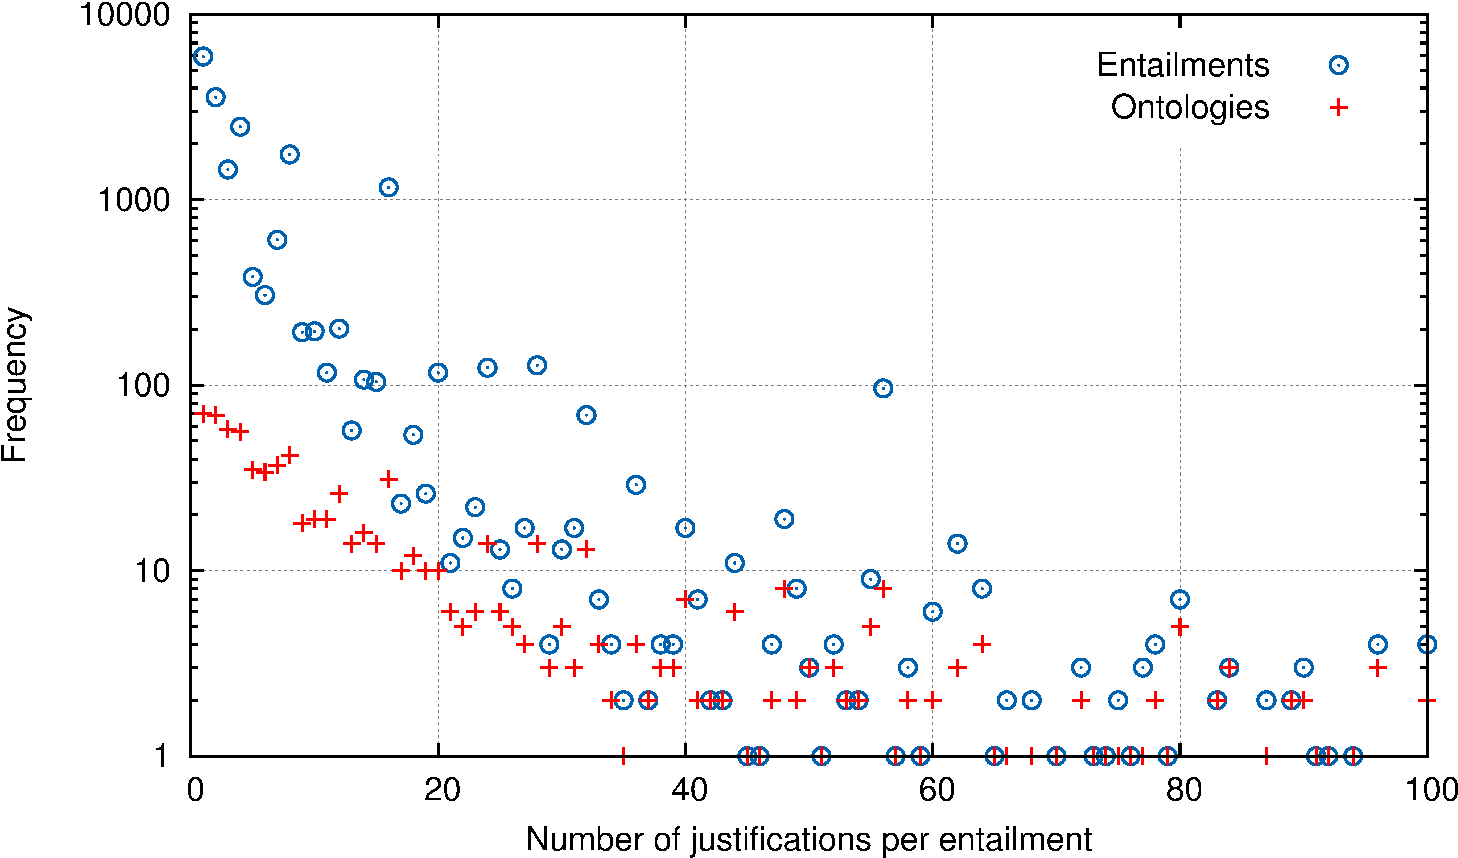
\includegraphics[width=14cm]{plots/frequency.pdf}
\caption{Frequency of multiple complex justifications in the corpus.}
\label{fig:frequency-justperent-nonself-sat}
\end{figure}

In $S_{u}$, the average number of justifications per entailment is 24.1 (\sdev = 12.8, \median = 32), with a maximum of 55 justifications for entailments in the \emph{Quantitative Imaging Biomarker} ontology. 7 of the 10 ontologies contain only entailments with exactly 1 justification, whereas the remaining 3 ontologies contain only entailments with multiple justifications. 

While we might expect to see a correlation between the size of an ontology and the number of complex justification it generates, we found that there are no obvious indicators for the occurrence of multiple justifications in an ontology. The Spearman rank coefficient\footnote{A coefficient $\rho$ of +1 (-1) indicates a strong positive (negative) correlation between two variables, whereas a $\rho$ of 0 indicates no correlation.} $\rho = 0.09$ ($p = 0.43$) indicates no correlation between the number of logical axioms in an ontology in set $S_{s}$ and the number of justifications per entailment. Due to the small number of ontologies in $S_{u}$, the correlation analysis was only performed for $S_{s}$.

\paragraph{Ontology activity and axiom power}

The 145,689 complex justifications in $S_{s}$ contain a total of 22,371 axioms. On average, one fifth of the axioms in an ontology (22.2\%, \sdev = 20.4\%, \median = 15.1\%) are active in  complex justifications for their entailed atomic subsumptions, with some ontologies having as many as 75.5\% of their axioms participating in justifications. Note that the small number of axioms compared to the number of justifications indicates a high amount of shared axioms in the corpus; we will focus on the matter of axiom overlap below.

Intuitively, we would expect to see an obvious correlation between the number of entailments in an ontology and its activity (the proportion of active axioms), since more entailments would imply more justifications and axioms occurring in them; this is somewhat confirmed by $\rho = 0.49$ (Pearson's correlation coefficient) indicating a weak linear correlation ($p < 0.001$).


\paragraph{Graph components}
In order to determine the overall connectedness of justifications, we consider the number of connected components in each j-graph. On average, each graph contains 4.6 (\sdev=9.8, \median=2) connected components, but almost half of the graphs in $S_s$ (37 out of 78) consist of exactly one component. The largest number of components can be found in the \emph{International Classification for Nursing Practice} ontology, which has 1,063 complex justifications for 762 entailments that are split up over 68 components.

As we have mentioned in previous chapters, the justification finding algorithm uses the Hitting Set Tree algorithm, which depends on optimisations such as justification reuse. This implies that largely disjoint justification sets may have a negative impact on the performance of the \enquote{find all} algorithm. However, there seems to be no correlation between the number of components in a j-graph and the average time required to find a justification ($\rho$ = 0.13, $p = 0.25$), or the number of components and the number of calls to the \enquote{find one} subroutine ($\rho$ = 0.06, $p = 0.58$).\footnote{Note, however, the high p-values which indicate that these findings are not statistically significant.}


\subsection{Justification overlap}

\paragraph{Inferential power of justifications}

While multiple justifications per entailment occur very frequently in the corpus, the number of justifications with multiple entailments is comparatively low, with only 709 justifications in $S_{s}$ having out-degrees $\geq2$ in the j-graph. On average, a justification in $S_{s}$ has 1.1 entailments (\sdev = 2.2, \median = 1), with a maximum of 120 entailments for 16 fairly small justifications (containing 5 to 7 axioms) in the \emph{SNP} ontology. Across the corpus, only 17 out of the 78 ontologies contain justifications with multiple entailments.

There is no correlation between the size of a justification and its number of entailments ($\rho$ = -0.07, $p < 0.001$). The average size of justifications that have only one entailment is 7.9, with some of the largest justifications (20 and more axioms) having only one entailment, whereas the average size of a justification with multiple entailments is 4.2 axioms.


\paragraph{Axiom frequency and impact}

Regarding the frequency and impact of the axioms in the corpus, we want to find out how frequently axioms occur in multiple justifications, and how many entailments these axioms affect. On average, an axiom occurs in 51.3 justifications (\sdev = 242.1, \median = 5) in set $S_{s}$, with some key axioms in several ontologies occurring in thousands of justifications. Figure \ref{fig:arityimpact} shows the axiom frequency plotted against the average impact, following approximately a linear distribution as shown by the linear trendline.\footnote{Again, the \enquote{long tail} of the plot of up to 7,343 justifications has been cut off for presentation purposes.} 

\begin{figure}[tb]
\centering
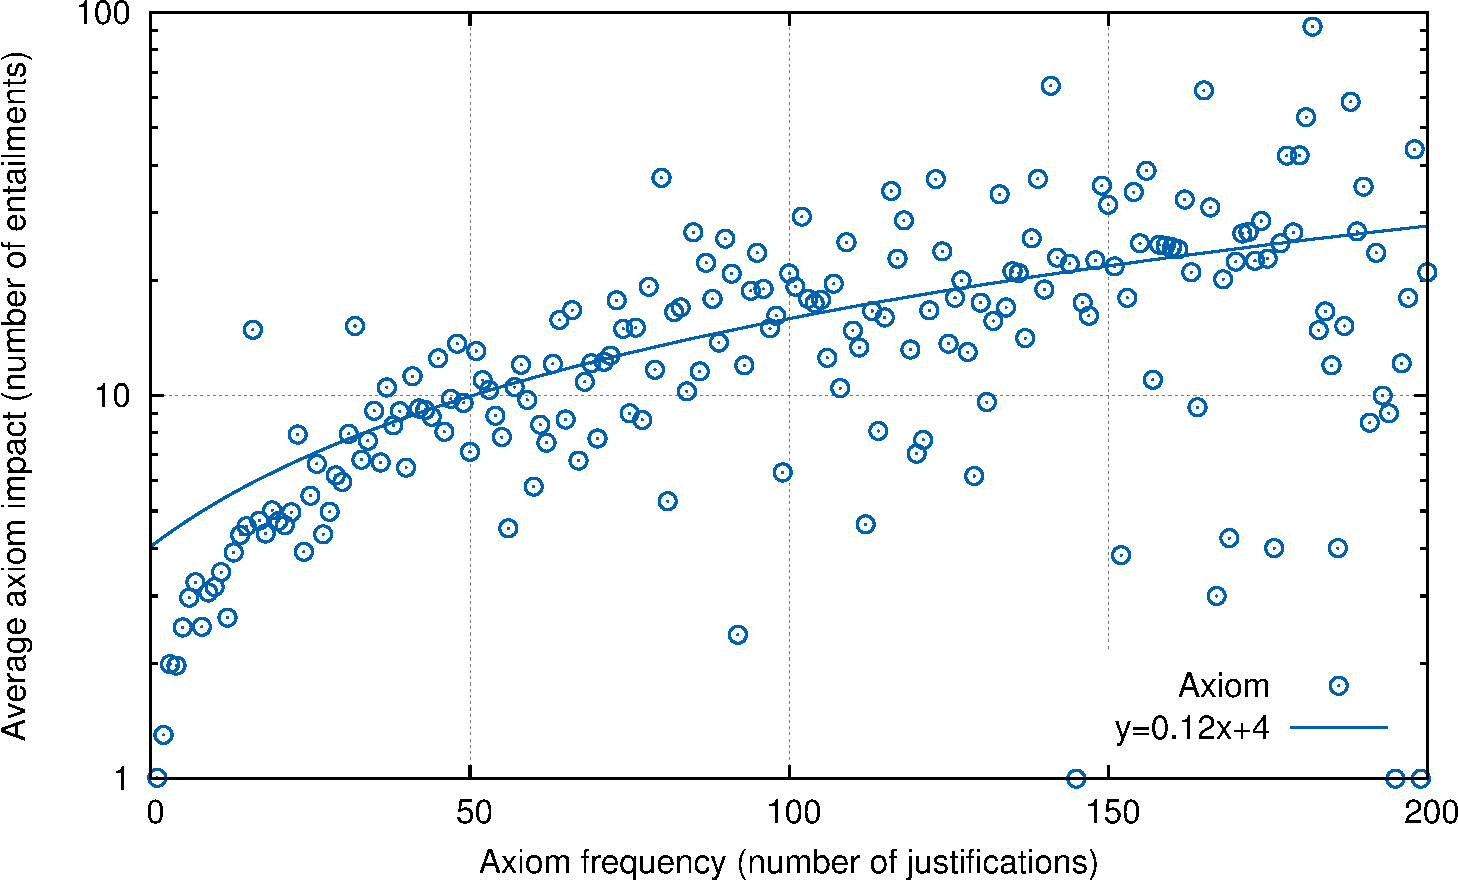
\includegraphics[width=14cm]{plots/arityimpact.pdf}
\caption[Axiom frequency vs average axiom impact.]{Axiom frequency vs average axiom impact, fitted with a linear trendline.}
\label{fig:arityimpact}
\end{figure}

The closeness of axiom frequency and impact is not surprising, since we have already seen that most justifications in the corpus only have a single entailment; therefore, the impact for most axioms is less than (if they occur in justifications for the same entailment) or equal to (if they occur in justifications for different entailments) the number of justifications they occur in. 

Interestingly, all the ontologies in the corpus (even those which contain only small numbers of justifications) contain some axiom which occurs in multiple justifications, and 23 ontologies contain some axiom which occurs in over 50\% of the justifications in the ontology. On average, the one axiom with the highest frequency in an ontology occurs in 36.3\% of all justifications of an ontology. 

An example of such a high-frequency axiom is the simple atomic subsumption \ax{Disease \subcls Disposition} which is used in 3,119 (96.5\%) of the 3,232 justifications in the \emph{NIF Dysfunction} ontology and affects 423 entailments. Another example is the domain axiom \ax{domain(measuredBy, MentalConcept)} in the \emph{Cognitive Atlas} ontology, which occurs in 92.5\% of the 830 justifications for 126 entailments.



\paragraph{Root and derived justifications}
Root and derived relationships occur frequently across the corpus: 73.4\% of the justifications in $S_{s}$ are derived, and 7.4\% of the justifications are root justifications which have derived justifications. The remaining 19.2\% are root justifications that do not have any justifications that are derived from them, that is, they are either additional independent justifications for derived entailments, or justifications for entirely independent root entailments. Table \ref{tab:rootderived} gives an overview of the root and derived relationships in the corpus; root justifications that are subsets of derived justifications are denoted by $Justs_{rsub}$, root justifications that are no subsets are denoted by $Justs_{r}$, and derived justifications are denoted by $Justs_{d}$.

\begin{table}
\centering
\caption[Root and derived justifications in $S_{s}$ and $S_{u}$.]{Root and derived justifications in $S_{s}$ and $S_{u}$, in number of justifications and proportion of the total.}
\label{tab:rootderived}	
\begin{tabu}{lrrrrrrr}
\toprule
&  & \multicolumn{2}{c}{$Justs_{rsub}$} & \multicolumn{2}{c}{$Justs_{d}$} & \multicolumn{2}{c}{$Justs_{r}$}\\
\cmidrule(r){3-4} \cmidrule(r){5-6} \cmidrule(r){7-8}
Set		& Total & Count & \% & Count & \% & Count & \% \\
\midrule
$S_{s}$ & 145,689 & 10,723 & 7.4\% & 107,002 & 73.4\% & 27,964 & 19.2\% \\
$S_{u}$ & 10,352 & 115 & 1.1\%  & 10,184 & 98.4\% & 53 & 0.5\% \\
\bottomrule 
\end{tabu} 
\end{table}

Looking at the repair impact of root justifications, we find that a justification in $Justs_{rsub}$ has 17 justifications on average which are derived from it (\sdev = 92.8, \median = 3), and 5.4 entailments (\sdev = 19.5, \median = 2) that are entailed by these derived justifications. In other words, while a root justification may have a fairly large number of justifications (17) that are derived from it, the number of entailments that can be repaired by fixing a single root justification is comparatively low (5.4).

The subset relationship between root and derived justifications is also visible in the size of justifications: on average, a root justification contains 4.7 axioms, whereas a derived justification has a size of 8.4 axioms. 7.6\% of the root justifications are indeed single axiom justifications which occur in a large number of derived justifications. However, while we may expect a small justification to be more likely to be contained in derived justifications, there is only a weak correlation between the size of a root justification and the number of justifications that are derived from it ($\rho = -0.26, p < 0.001$).

70 of the 78 ontologies in $S_{s}$ contain some derived justifications. 6 of of the 8 remaining ontologies only contain very small numbers of justifications, which do not lend themselves to subset relationships, whereas the \emph{Cancer Research and Management} ontology and \emph{Gene Ontology Extension} contain no derived justifications despite having 348 and 6,421 justifications, respectively.

In the set $S_{u}$, the effect of root and derived justifications is even more pronounced: 98.4\% of the justifications are derived from only 1.1\% of the justifications, and the remaining 0.5\% are root justifications which have no derived justifications. On average, a root justification has 88.6 derived justifications (\sdev = 208.6, \median = 2) which have 48.8 entailments (\sdev = 109.3, \median = 2). Note how this stands in contrast to the rather small number of entailments (5.4) that depend on root justifications in $S_{s}$. 5 of the 10 ontologies in $S_{u}$ contain root and derived unsatisfiable classes, whereas the remaining 5 ontologies contain only very few unsatisfiable classes (up to 4) at all.


\paragraph{Arbitrary overlap}

In order to determine the numbers and sizes of justification overlaps with more than a single axiom, we applied the Formal Concept Analysis (FCA) \cite{ganter05ar} \enquote{next concept} algorithm to the j-graphs in sets $S_{s}$ and $S_{u}$. This algorithm (often simply referred to as \enquote{Ganter's algorithm}) provides an efficient means for computing the largest shared axiom sets between justifications. The ToscanaJ FCA framework\footnote{\url{http://toscanaj.sourceforge.net/}} includes a straight-forward implementation of Ganter's algorithm, which we used for overlap detection. Using the FCA algorithm, the justifications correspond to the \emph{objects} in a  context, and the axioms correspond to the \emph{attributes}. Due to performance issues, the experiment was restricted to a random sample of maximum 5,000 edges per graph. 

\begin{figure}
\centering
		\begin{subfigure}{0.5\textwidth}
                \centering
                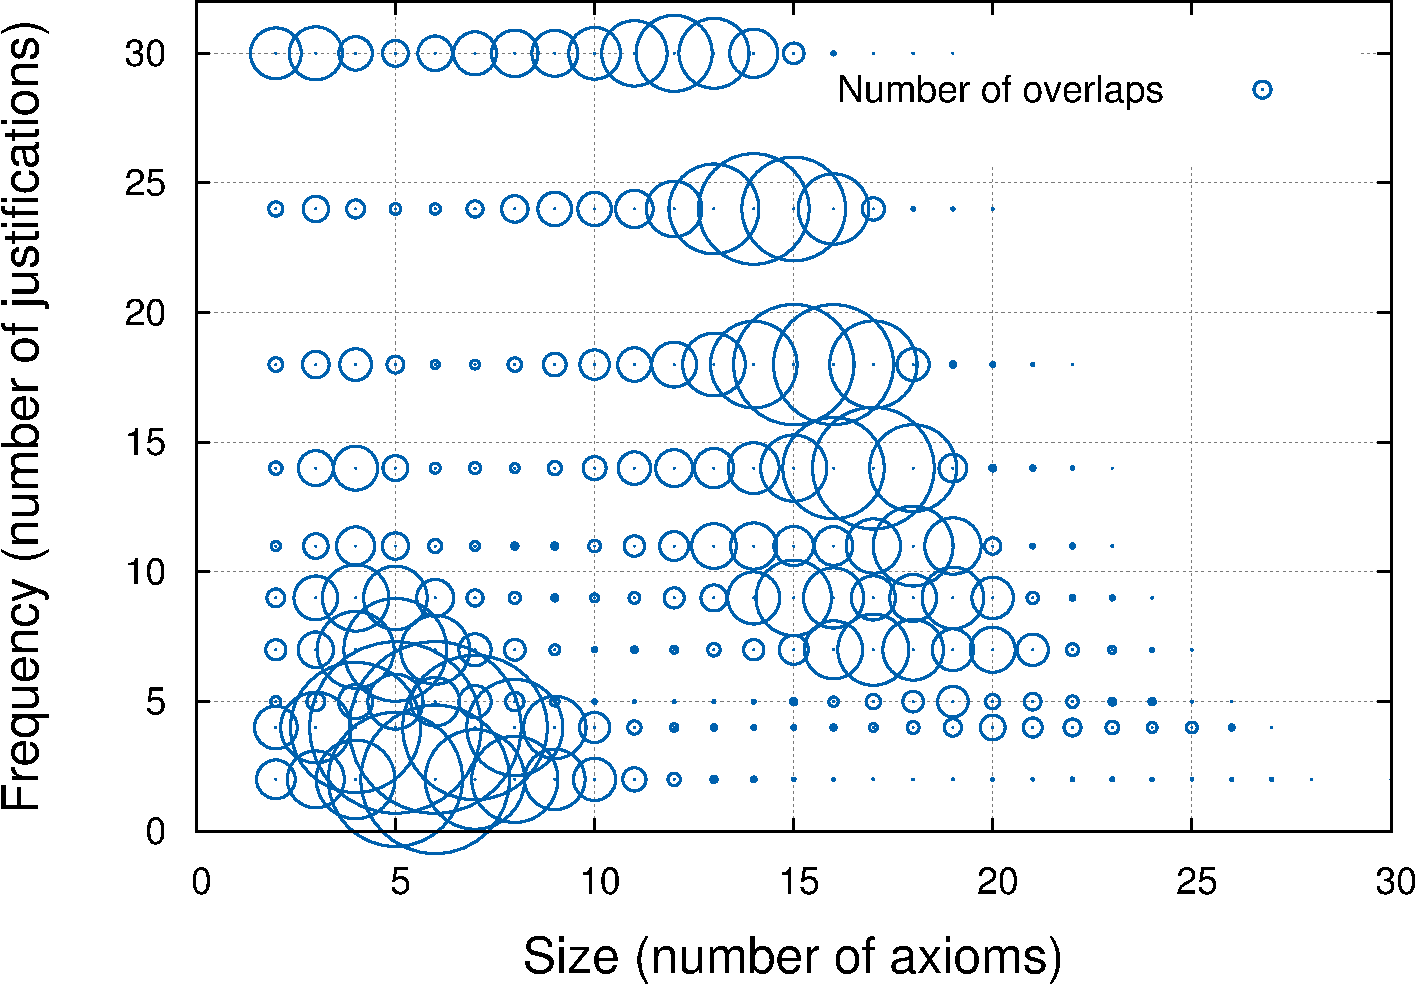
\includegraphics[height=5.2cm]{plots/overlap-count-all.pdf}
                \caption{Overlap frequency for \textbf{all} ontologies \\in $S_{s}$.}
        	\label{fig:overlap-all}
        \end{subfigure}%
         %add desired spacing between images, e. g. ~, \quad, \qquad etc. 
          %(or a blank line to force the subfigure onto a new line)
		\begin{subfigure}{0.5\textwidth}
                \centering
                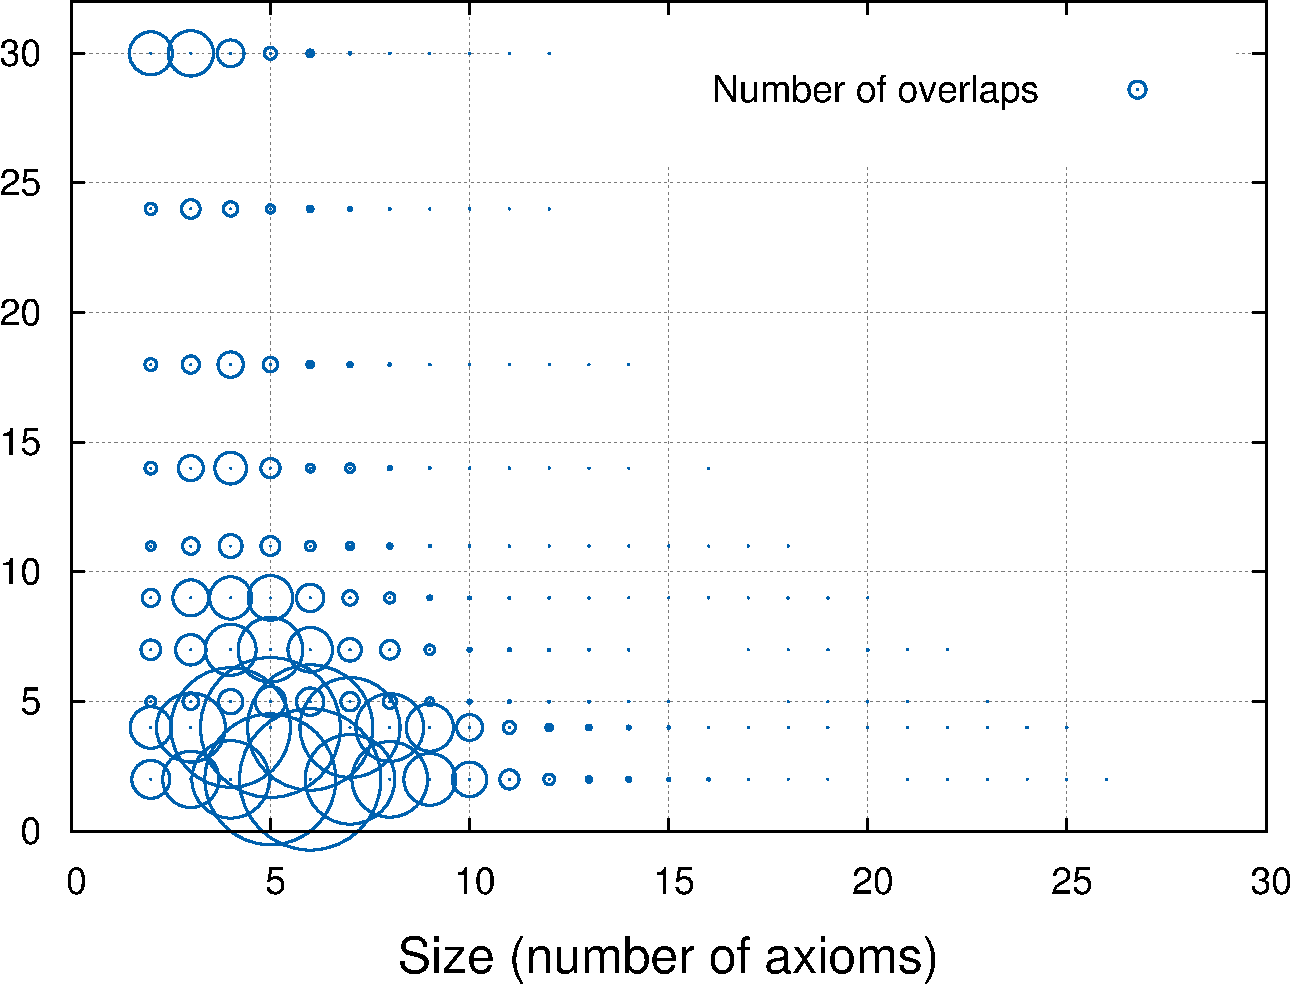
\includegraphics[height=5.2cm]{plots/overlap-count-reduced.pdf}
                \caption{Overlap frequency \textbf{excluding} \emph{Amino Acid} and \emph{Basic Vertebrate Anatomy}.}
        	\label{fig:overlap-reduced}
        \end{subfigure}
        \caption[Overlap frequency with and without outlier ontologies.]{Overlap frequency with and without outlier ontologies. Bubble size indicates frequency.}
\end{figure}

Across the ontologies in $S_{s}$, overlaps between justifications occur frequently, with an average size of 10.8 shared axioms (\sdev = 5.7, \median = 11) and an average frequency of 11.9 justifications (\sdev = 11.8, \median = 9) that the shared axiom set occurs in, i.e.\ on average, 11.9 justifications share the same axiom set. Figures \ref{fig:overlap-all} and \ref{fig:overlap-reduced} show the frequency of overlap of different size and frequency across the corpus including and excluding the two ontologies which contribute the largest numbers of overlaps. For presentation purposes, the values on the y-axis (i.e.\ the number of justification an overlap of a certain size occurs in) were binned in 10th percentile steps, leading to all overlaps with a frequency greater than 24 falling into the top-most bin. 

The plot shows that the majority of overlaps (i.e.\ the largest bubbles) have a size of around 5 axioms and occur in up to 5 justifications. However, there are also overlapping cores of around 15 to 20 axioms which occur fairly frequently in up to 18 justifications; as we can see if we compare \ref{fig:overlap-all} to \ref{fig:overlap-reduced}, these large, high-frequency overlaps are almost exclusively contributed by the \emph{Amino Acid} and \emph{Basic Vertebrate Anatomy} ontologies. If we exclude these two ontologies from the set, the overlaps are reduced to an average of 5.5 axioms (\sdev = 2.5, \median = 5) and a frequency of 7.8 justifications (\sdev = 14.3, \median = 4).

Nearly all ontologies in $S_{s}$ (75 out of 78) contain at least some overlapping justification subset, with two ontologies standing out as extreme outliers.  The \emph{Amino Acid} ontology contributes over half of the found overlaps in the corpus, which is rather surprising, as with 112 entailments, 477 axioms, and a description logic expressivity of \dl{ALCF}, this ontology could be considered fairly inexpressive.

However, if we take a closer look at the \emph{Amino Acid} ontology, we find that it contains an axiom of the type \ax{AminoAcid \eqcls A \disj C \disj D \ldots \disj Y} with 20 named classes in the disjunction. This axiom, in turn, leads to a large number of justifications (2,652) containing subsumption axioms for each operand in the disjunction, plus a small number of \enquote{bridging} axioms that cause the entailment to hold. For 1,782 of the 2,562 justifications, this axiom pulls in a large core of up to 29 other axioms, thus leading to the large numbers of overlaps observed in the ontology.

A similar effect can be seen in the \emph{Basic Vertebrate Anatomy} ontology, another fairly small ontology (99 classes, 386 axioms, \dl{SHIF}) which, however, has a high number of object properties (74 compared an average of 22.2). The ontology contains a number of axioms describing the relations between its object properties as part-whole relationships, such as \ax{has\_subdivision \subcls has\_determinate\_part} and \ax{is\_subdivision\_of \eqcls \inv{has\_subdivision}}. Again, these property axioms pull in other \enquote{bridging} axioms which leads to cores of up to 17 axioms occurring in large numbers of justifications.

Both of these outlier ontologies have high degrees of overlaps between multiple justifications for \emph{single} entailments, but only small numbers of overlaps between justifications for several different entailments. This agrees with the general trend in the corpus, where on average those  justifications which do share an overlap only have between 1 and 2 entailments (mean = 1.9, \median = 1, \sdev = 5.1). In other words, overlap tends to occur mainly between justifications for the \emph{same} entailment.


\subsection{Justification isomorphism}

In order to determine the frequency of isomorphic justifications in the corpus, we analysed the complex justifications for the entailments in set $S_{s}$ and $S_{u}$ in three different experiments: 
\begin{compactenum}
\item justifications for a \emph{single} entailment.
\item justifications for \emph{all} entailments within an ontology.
\item justifications for \emph{all} entailments of all ontologies across the corpus.
\end{compactenum}
The isomorphism statistics were generated for all three types of isomorphism, that is, strict, subexpression-, and lemma-isomorphism. 

Due to performance issues, justifications containing more than 10 axioms or conjunctions/disjunctions with more than 5 operands were excluded from this part of the study. This excluded some dominant justifications (such as those containing the large disjunction axiom in the \emph{Amino Acid} ontology mentioned above), but still resulted in a set of 141,560 justifications for 19,097 entailments in $S_{s}$, which is an average of 7.4 justifications per entailment (compared to 7.8). Note that this also means that the total numbers of justifications given in this section for some of the ontologies will differ from the number of complex justifications listed in the overview table in Appendix A.

The mean times required to determine isomorphism between justifications for each of the three types (including parsing the justifications and existing templates from file) are listed in Table \ref{tab:iso-times}. Note that the experiments for the three isomorphism types were run in parallel, which could potentially cause a drop or fluctuations in performance (as the \enquote{Within ontology} times for strict versus subexpression-isomorphism show). Furthermore, the checks within ontologies and across the corpus each reuse the templates found in the previous stage, which drastically reduces the number of comparisons that have to be carried out. 

\begin{table}[htb]
\centering
\caption{Mean times (in seconds) per ontology for isomorphism detection.}
\label{tab:iso-times}	
\begin{tabu}{lrrrrrr}
\toprule
 Size & Iso  & S-iso & L-iso\\
\midrule
Individual entailments 	&	22.8	&  48.5	& 100.8  \\
Within ontology 		&	103.8	&  99.2	& 192.3  \\
Across corpus 			&	24.6	&  42.3 &  97.7 \\
\bottomrule 
\end{tabu} 
\end{table}


\subsubsection{Individual entailments}

\paragraph{Strict isomorphism}
Due to restrictions on the types of justifications used in the isomorphism experiments, the number of justifications for the entailments in this subset of $S_{s}$ is marginally lower than in the j-graph analysis, with an average of 7.4 justifications per entailment. Strict isomorphism reduces this number to an average of 4.9 templates per entailment (\sdev = 9.5, \median = 2), which is a reduction by 33.7\% compared to the full corpus.

On average, a template covers 1.5 justifications (\sdev = 2.3, \median = 1), with some ontologies containing entailments with large numbers of isomorphic justifications. One such example is the \emph{Orphanet Ontology of Rare Diseases}, whose dominating templates are of the type
\begin{align*}
\Theta_{1} =\{\dlax{C1 \subcls C2}, \dlax{C2 \subcls \exists p1.C4}, \dlax{domain(p1, C3)} \} \models \dlax{C1 \subcls C3}
\end{align*}
with atomic subsumption chains of arbitrary size in place of the first subsumption axiom, and some variations that include subproperty axioms. Two of the templates of this type cover the majority (110 and 105 justifications, respectively) of the 220 justifications each for several entailments in the ontology. From personal contact with the \emph{Orphanet} developers we have learned that this OWL ontology is in fact generated automatically from an existing medical database, which explains the frequent occurrences of uniform justifications.


\paragraph{Subexpression-isomorphism}

Subexpression-isomorphism across the justifications of individual entailments only affects a very  small number of entailments in the corpus. The average number of templates per entailment, compared to the full corpus, remains the same when rounded,\footnote{The precise number of templates is 4.915 for strict and 4.903 for subexpression-isomorphism.} at 4.9 templates per entailment (\sdev = 9.5, \median = 2). Compared to strict isomorphism, the number of templates is reduced by only 0.3\%. This small reduction does not affect the average number of justifications per entailment, which remains the same at 1.5 justifications.

Only 166 entailments (0.9\% of the total corpus) from 15 of the 78 ontologies are affected by subexpression-isomorphism; the remaining 63 ontologies contain the same number of templates as for strict isomorphism. For those ontologies that are affected, the decrease in templates compared to strict isomorphism is an average of 19.8\%, reaching up to 50\% for 9 entailments in the \emph{Bleeding History Phenotype} ontology.

\paragraph{Lemma-isomorphism}

While subexpression-isomorphism does not have a strong effect on individual entailments, lemma-isomorphism shows a more visible reduction in template numbers.\footnote{Note that $S_{s}$ and $S_{u}$ do not contain any justifications that consist entirely of atomic subsumption chains. That is, all atomic subsumption chains that are affected by l-isomorphism will be strict subsets of the complex justifications in the corpus.} On average, the justifications are reduced to 4.7 templates per entailment (\sdev = 8.8, \median = 2), which is reduction by 4.1\% compared to both strict and subexpression-isomorphism.

A total of 1,492 entailments (7.8\% of the total corpus) from 43 ontologies are affected by lemma-isomorphism, with an average reduction of 30.3\% compared to strict isomorphism for those entailments. The strongest effects can be seen in the \emph{Fission Yeast Phenotype} ontology, where the justifications for several entailments only differ in the length of their atomic subsumption chains and thus are each reduced to a single template of the type \begin{align*}
\Theta_{2} = \{\dlax{C1 \subcls \ldots \subcls C_{n}, C_{n} \eqcls C2 \conj \ldots} \} \models \dlax{C1 \subcls C2}.
\end{align*}


\subsubsection{Isomorphism within ontologies}

Across the justifications for all entailments of an ontology, the reductions caused by the three equivalence relations are more clearly visible than for individual entailments. Figure \ref{fig:iso-comparison} shows an overview of the effects of the different isomorphism types for the 25 ontologies containing the largest numbers of justifications in the corpus. Each cluster represents an ontology, with the ontologies ordered by the number of justifications they contain. Each bar in a cluster represents the reduction compared to the previous equivalence relation (that is, we compare strict isomorphism with the full set of justifications, s-isomorphism with strict isomorphism, and l-isomorphism with s-isomorphism). We can see that the effects of the relations differ strongly across the ontologies, with strict isomorphism generally having the strongest impact, and subexpression-isomorphism having the lowest impact.

Overall, only three ontologies show no effect for \emph{any} of the three types of isomorphism; two of these contain only a single justification (which means there is no reduction possible), while one ontology (\emph{OBOE SBC}) contains 5 distinct justifications.


\begin{figure}
\centering
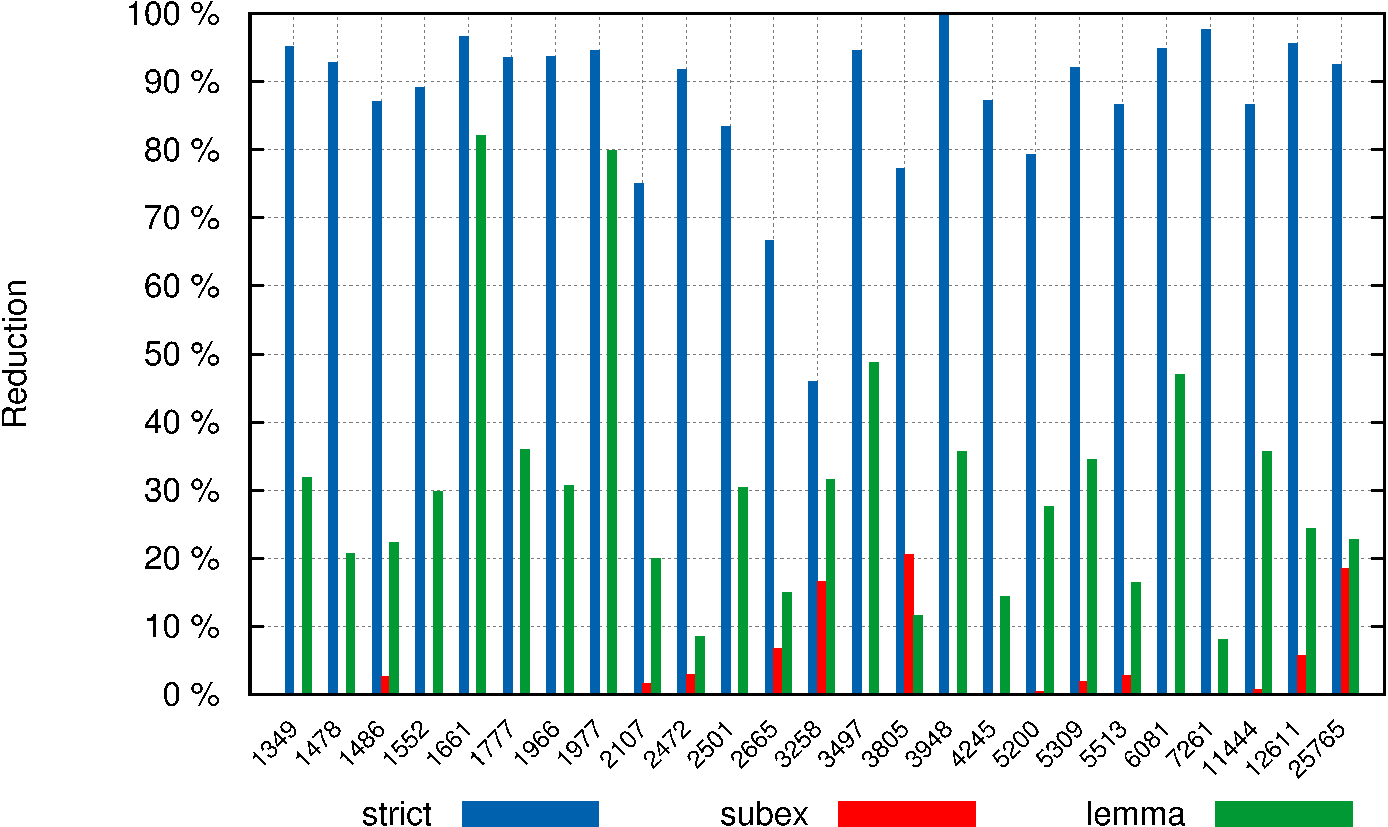
\includegraphics[width=14cm]{plots/iso-comparison.pdf}
\caption[Comparison of reduction caused by isomorphism types.]{Comparison of reduction caused by isomorphism types. Each cluster represents an ontology. Ontologies are ordered by number of justifications.}
\label{fig:iso-comparison}
\end{figure}


\paragraph{Strict isomorphism}

Compared to the results for individual entailments, the effects of the equivalence relations are much more significant if we consider the justifications for \emph{all} entailments in an ontology. On average, an ontology in $S_{s}$ contains 1,814.9 justifications; these are reduced to 436.1 templates through strict isomorphism, which is an average reduction by 73.1\%.

4 ontologies with small numbers of justifications (less than 10) are not affected by strict isomorphism, while the remaining 74 ontologies show reductions of up to 99.6\%. Even more strikingly, 28 of the ontologies are reduced to less than 10\% of their justification corpus. With an average number of 3,092 justifications per ontology, these reductions reveal significant numbers of structurally similar justifications.

The templates cover an average of 8.2 justifications each (\sdev = 22.4, \median = 2), with some of the highest coverage occurring in the \emph{Orphanet} ontology. The 3,948 justifications in this ontology can be reduced to only 14 templates, which are all variations (featuring atomic subsumption chains of varying length) of the template $\Theta_{2}$ we have shown above.


\paragraph{Subexpression-Isomorphism}

Subexpression-isomorphism reduces the justifications in the corpus by an average of 74\% per ontology, which is only a small change (0.9\%) compared to strict isomorphism. The number of justifications covered by a single template is slightly increased to 8.8 (\sdev = 23.5, \median = 2) justifications per template.

Again, the majority of ontologies (44 of 78) are not affected by subexpression-isomorphism, whereas 5 ontologies show reductions of between 20\% and 38.3\% compared to strict isomorphism. This includes the \emph{Bleeding History Phenotype} ontology (1,158 justifications, 60 isomorphism templates, 37 s-isomorphism templates), which contains a number of justifications of the type
\begin{align*}
\{ \dlax{C1 \subcls \exists p1.(C2 \disj C3)}, \dlax{domain(p1, C4)} \} \models \dlax{C1 \subcls C4}
\end{align*}
which is subexpression-isomorphic to justifications which contain a named class in place of the disjunction $C2 \disj C3$ in the subsumption axiom, thus matching template $\Theta_{1}$.

Closer inspection of the \emph{Lipid} ontology (3,258 justifications as shown in Figure \ref{fig:iso-comparison}, 1,762 isomorphism templates, 1,471 s-isomorphism templates) reveals that a large number of justifications in the ontology consist of a single equivalence axiom of the form \dlax{C1 \subcls C2 \conj x} with the entailment being \dlax{C1 \subcls C2}. The remainder of the conjunction, represented by $x$, consists of a number of complex expressions of varying length and nesting depth. While s-isomorphism captures these types of justifications (since the remainders $x$ can all be matched against each other), the actual reason for their similarity lies in their identical \emph{cores} \dlax{C1 \subcls C2}, with the remainder $x$ being a superfluous part.

\paragraph{Lemma-isomorphism}

As for single entailments, lemma-isomorphism has a more significant effect on the justification corpus than subexpression-isomorphism when applied across each ontology. L-isomorphism reduces the justifications in an ontology by an average of 78.2\%, which is a 4.2\% difference compared to subexpression-isomorphism. 

A template covers an average of 12 justifications (\sdev = 38, \median = 3) in each ontology, which is a visible increase from the 8.8 justifications covered by subexpression-isomorphism. 13 ontologies (with an average number of 32.1 justifications) show no reaction to l-isomorphism, whereas 12 ontologies containing large numbers of justifications (mean = 1,555.8) see a reduction of 41.7\% and more, up to 82.1\% compared to subexpression-isomorphism.

\subsubsection{Isomorphism across the corpus}

In the final stage of our analysis of isomorphism in the BioPortal corpus, we will look at the templates spanning all justifications for all entailments across the ontologies in the corpus. While we have seen that isomorphic justifications occur frequently within an ontology, we now analyse the structural similarity of justifications across multiple ontologies. Table \ref{tab:iso-cross} gives an overview of the numbers of templates in $S_{s}$ for the three isomorphism types against the full justification corpus, as well as the coverage (number of justifications) per template.

\begin{table}
\centering
\caption{Template frequency and coverage across the corpus.}
\label{tab:iso-cross}
\begin{tabu}{lrrrrrr}
\toprule 
		& 			& 		&  \multicolumn{4}{c}{Coverage} \\
\cmidrule(r){4-7}
Type & Count & \% of $S_{s}$ &  Mean & Median & Min & Max \\
\midrule 
all 	& 141,560 	& 100\% 	& - 		&  - 	& - & - \\
strict 	& 12,527 	& 8.8\%  	& 11.3  	&  2 	& 1 & 2,072 \\
subex 	& 10,952 	& 7.8\%  	& 12.9 		&  2	& 1 & 2,128  \\
lemma 	& 5,487  	& 3.1\%    & 25.8 		& 3 	& 1 & 7,490      \\
\bottomrule 
\end{tabu} 
\end{table}

\paragraph{Strict isomorphism}

The 141,560 justifications in $S_{s}$ are reduced to only 12,527 templates, which is a reduction by 91.2\%. On average, 11.3 justifications (\sdev = 54.3, \median = 2) share the same template, with the 8 most frequent templates covering over 1,000 justifications each. The most frequent templates (by numbers of justifications covered) are all variations of the template $\Theta_{1}$, that is, a combination of a domain axiom and a subsumption axiom with an existential restriction on the RHS, including some additional subsumption axioms, an equivalence axiom in place of a subsumption, or variations of the filler.

Nearly half of all templates (41.3\%) in the corpus cover exactly one justification in a single ontology. We might larger templates to be more \enquote{specific} to a particular ontology, thus covering fewer justifications overall, and conversely, a smaller template might be more \enquote{generic}, thus covering more justifications. However, the size (number of axioms) of a template seems to be no indicator for the number of justifications it covers: the average size (7.3 axioms) of a template covering multiple justifications is only marginally lower than of those templates covering a single justification (7.5 axioms). 

If we look at the spread of templates across the ontologies in the corpus, we find that only 8.7\% of the templates cover justifications in multiple ontologies, with a maximum spread of 26 ontologies for two templates which are, again, variations of $\Theta_{1}$. Figure \ref{fig:iso-freq} shows the frequency distributions of the justification templates across the justifications and ontologies in $S_{s}$. The y-position of a data point indicates the number of justifications a template covers is, and the bubble size indicates the number of ontologies a template occurs in. 

We can see that a small number of templates covers large numbers of justifications, with a steep drop to 10 and less justifications per template around the 2,000 mark. If we take a closer look at the numbers, we find that the majority of justifications in the corpus (81.2\%) are covered by the 2,000 most frequent templates (out of 12,527), and a third (33.1\%) of justifications are even covered by the 100 most frequent templates.

\begin{figure}
\centering
		\begin{subfigure}{0.5\textwidth}
                \centering
                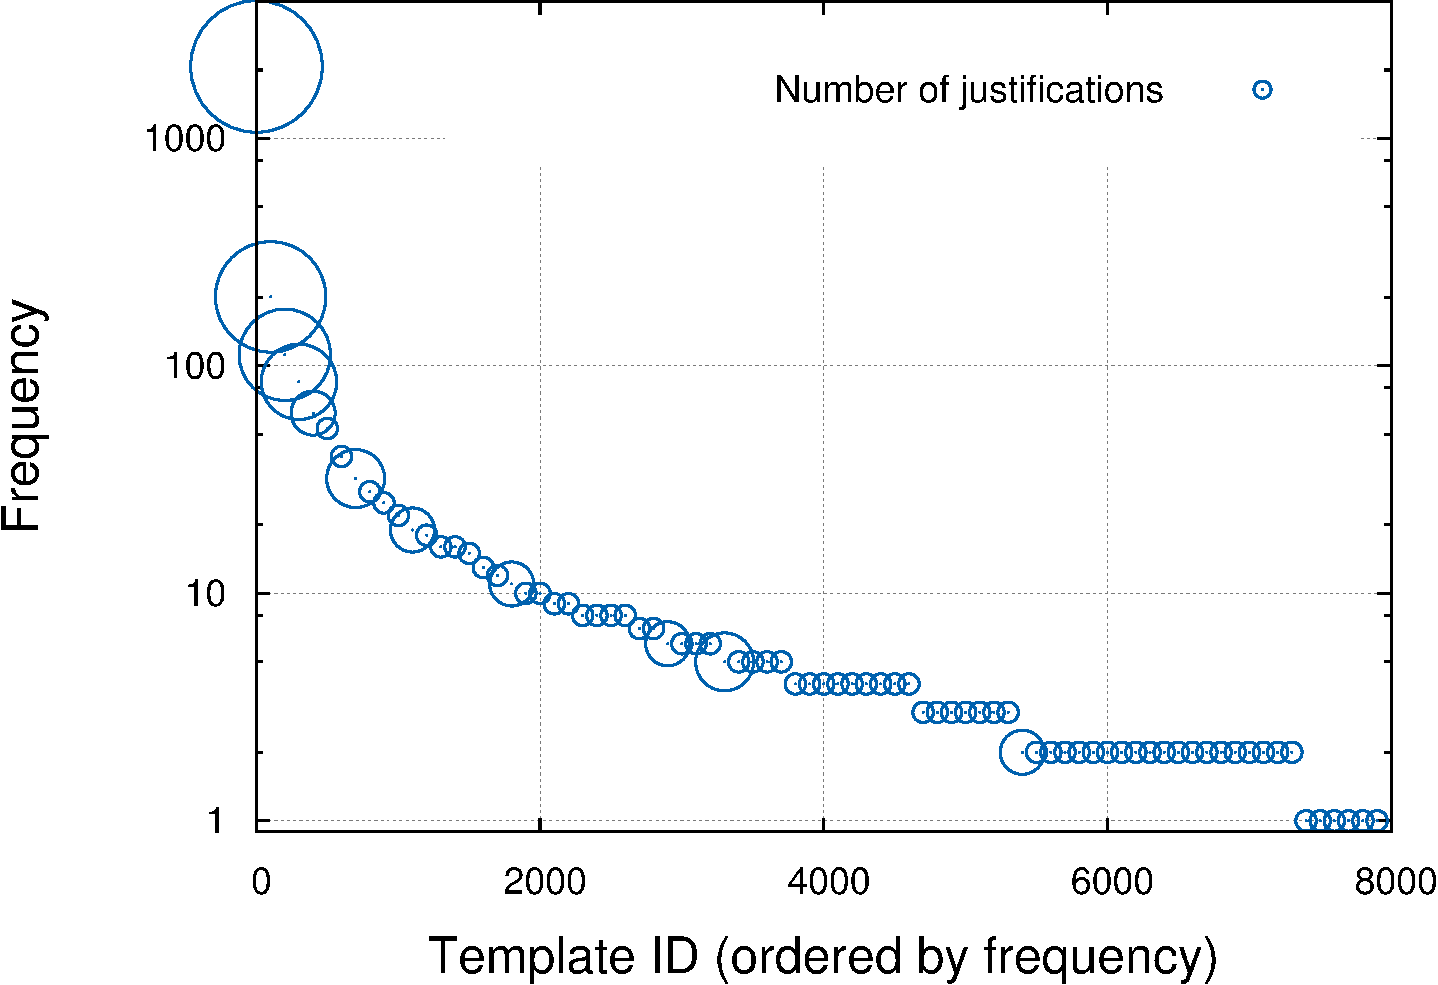
\includegraphics[height=5.2cm]{plots/iso-template-freq.pdf}
                \caption{Template frequency for strict iso.}
        	\label{fig:iso-freq}
        \end{subfigure}%
         %add desired spacing between images, e. g. ~, \quad, \qquad etc. 
          %(or a blank line to force the subfigure onto a new line)
		\begin{subfigure}{0.5\textwidth}
                \centering
                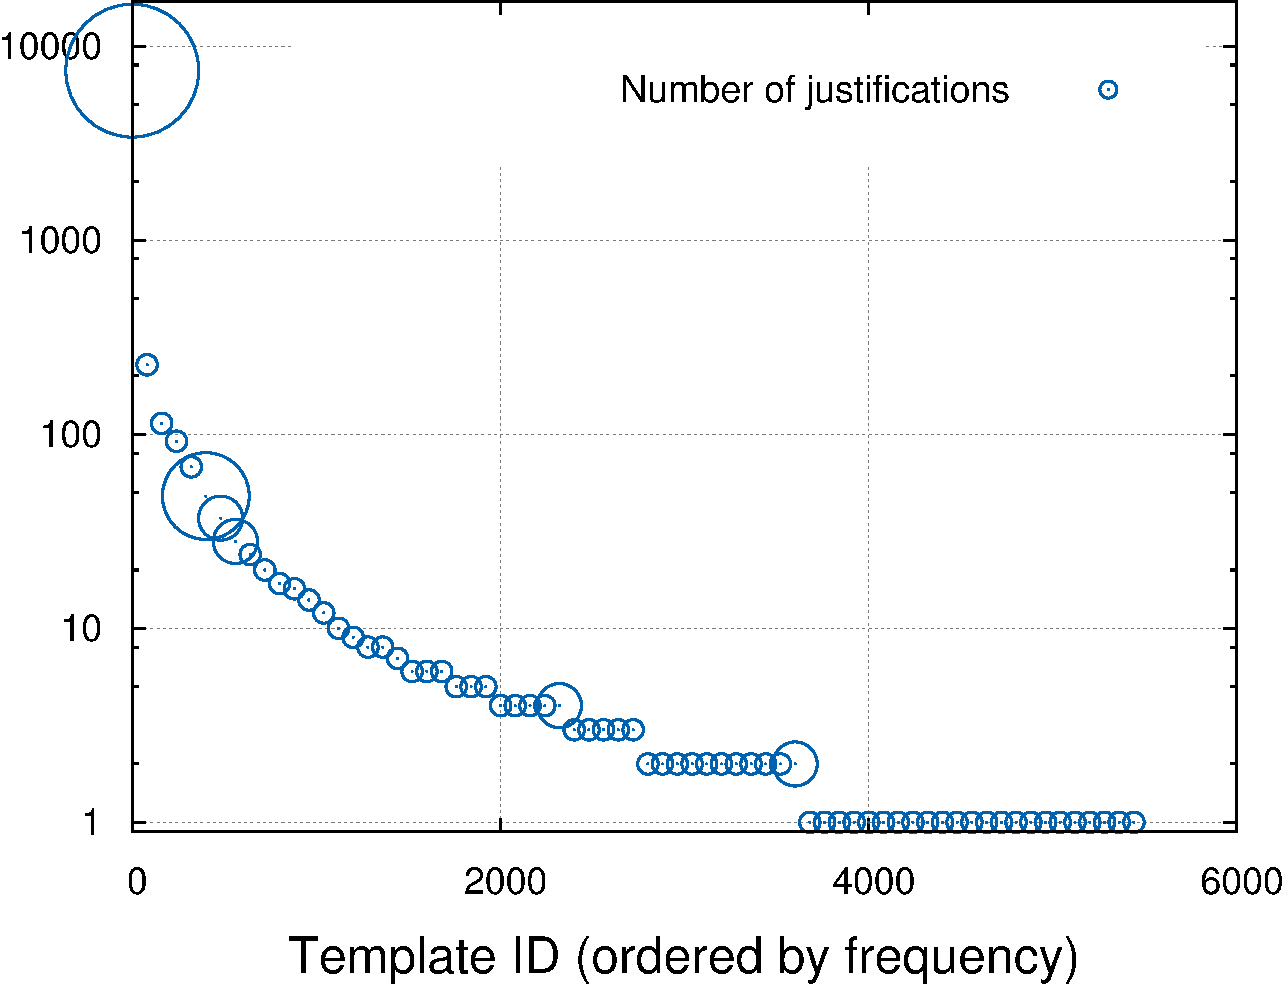
\includegraphics[height=5.2cm]{plots/iso-template-freq-lemma.pdf}
                \caption{Template frequency for l-iso.}
        	\label{fig:iso-freq-lemma}
        \end{subfigure}
        \caption{Template frequencies for strict and lemma-isomorphism.}
\end{figure}

\paragraph{Subexpression-isomorphism}
The effects of subexpression-isomorphism across the corpus are only marginal compared to strict isomorphism. The justifications are reduced to 10,952 templates, which is an overall reduction by 92.2\% and a 1\% difference compared to strict isomorphism. The number of justifications covered by a single template is slightly increased with an average of 12.9 justifications (\sdev = 59, \median = 2) per template.

The most frequent template (by numbers of justifications) is again $\Theta_{2}$, which covers 2,128 (1.5\% of the total set) justifications in 26 ontologies. Across the ontologies in the corpus, the most frequent template occurs in 28 of the 78 ontologies. This template is a single equivalence axiom which we have already seen in the \emph{Lipid} ontology:
\begin{align*}
\Theta_{3} = \{\dlax{C1 \eqcls C2 \conj x} \} \models \dlax{C1 \subcls C2}
\end{align*}
The superfluous part $x$ matches a number of operands such as atomic classes and existential restrictions. Interestingly, while this template occurs in the highest number of ontologies, it only covers 573 justifications across the corpus.


\paragraph{Lemma-isomorphism}

Across all justifications in the corpus, l-isomorphism has a clearly visible impact. The 141,560 justifications are reduced to only 5,487 templates, which is less than half as many templates as the strictly isomorphic ones, and an overall reduction of 96.9\%. Figure \ref{fig:iso-freq-lemma} shows the frequency of templates for lemma-isomorphism.

On average, a template covers 25.8 justifications (\sdev = 208.5, \median=3); however, the large standard deviation shows that the distribution of justifications per template has shifted towards a few very frequent templates, whereas there is still a \enquote{long tail} of 1,878 templates which match only a single justification. If we consider the distribution of justifications per template over the quartiles of the corpus, 25\% of the justifications in $S_{s}$ can be covered by the 8 most frequent templates, 50\% by the 44 most frequent templates, and 75\% by the 277 (out of 5,487) most frequent templates.

The most frequent templates, by number of justifications they cover, are all subtle variations of a template containing only two or three axioms. Some of these templates, alongside their frequencies (number of justifications the template covers and number of ontologies the template occurs in), are listed in Table \ref{tab:templates}.
\begin{table}
\centering
\caption[Most frequent templates for lemma-isomorphism across the corpus.]{Most frequent templates for lemma-isomorphism across the corpus. \#J = number of justifications, \#O = number of ontologies.}
\label{tab:templates}
\begin{tabu}{llrr}
\toprule 
ID & Template & \#J & \#O \\
\midrule 
$\Theta_{4}$ & $\{C1 \subcls C2, C3 \eqcls C2 \disj C4, C3 \subcls C5\} \entails C1 \subcls C5$ &  7,490 & 27 \\ 
$\Theta_{5}$ & $\{C1 \subcls C2, C5 \eqcls C2 \disj C3 \} \entails C1 \subcls C5$ &  6,425 & 28 \\ 
$\Theta_{6}$ & $\{C1 \subcls C2, C3 \eqcls C2 \disj C4 \disj C6, C3 \subcls C5\} \entails C1 \subcls C6$ & 6,135 & 26 \\ 
$\Theta_{7}$ & $\{C1 \subcls C2, C5 \eqcls C2 \disj C3 \disj C4\} \entails C1 \subcls C5$ &  4,206 & 25 \\ 
\bottomrule 
\end{tabu} 
\end{table}
Note that any subsumption axiom in the templates $\Theta_{4}$ through $\Theta_{7}$ corresponds to an atomic subsumption chain of arbitrary length.

If we look at the number of ontologies a template occurs in, the most frequent templates are $\Theta_{3}$ and $\Theta_{5}$, both of which can be found in 28 of the 78 ontologies in the corpus. However, as with strict and subexpression-isomorphism, only a fraction of the templates (8.5\%) occur in multiple ontologies, while the majority of templates (5,018 out of 5,487) can only be found in a single ontology.


\subsubsection{Isomorphism and superfluity}

As we have already seen in our discussion of subexpression-isomorphism, a justification can potentially be non-isomorphic only due to it containing superfluous subexpressions that do not contribute to the entailment.

In order to determine to which extent superfluous parts affect isomorphism, we computed the laconic versions for justifications in $S_{s}$, which resulted in a corpus $S_{sl}$ containing 47,667 laconic justifications, of which 31.6\% were now atomic subsumption chain justifications or even self-justifications. The number of laconic justifications is significantly lower compared to $S_{s}$ for two reasons: first, due to the high runtime of the laconic justification generation mechanism, some justifications could not be computed; hence, due to timeouts, the number of entailments in $S_{sl}$ is only 18,300 (compared to 19,097 in $S_{s}$). More striking, however, is the effect of removing superfluous expressions on the equality between justifications: multiple regular justifications for individual entailments frequently resulted in \emph{the same} laconic justification, which drastically reduces the number of justifications despite the difference in the number of entailments being only small. Table \ref{tab:lacvsreg} shows a comparison of the cross-corpus reductions for laconic and regular justifications in $S_{s}$ and $S_{sl}$, respectively.

\begin{table}
\centering
\caption{Comparison of reductions in $S_{s}$ and $S_{sl}$.}
\label{tab:lacvsreg}
\begin{tabu}{lrrrr}
\toprule 
		&  \multicolumn{2}{c}{$S_{s}$ (regular)} & \multicolumn{2}{c}{$S_{sl}$ (laconic)}\\
\cmidrule(r){2-3}\cmidrule(r){4-5}
Type & Count & \% of $S_{s}$ &  Count & \% of $S_{sl}$ \\
\midrule 
all 	& 141,560 	& 100\% 	& 46,667 	&  100\%  \\
strict 	& 12,527 	& 8.8\%  	& 3,653 	&  7.8\%  \\
subex 	& 10,952 	& 7.8\%  	& 2,036 	&  6.2\%   \\
lemma 	& 5,487  	& 3.1\%    	& 1,789 	&  3.8\%   \\
\bottomrule 
\end{tabu} 
\end{table}

Across $S_{sl}$, strict isomorphism reduces the justifications to 3,653 templates, which is a reduction to 7.6\% (compared with 8.8\% for the regular justifications in $S_s$). 8 out of the 10 most frequent templates (by number of justifications they cover) are atomic subsumption chains between 1 and 8 axioms. Interestingly, this also indicates that, despite the apparent complexity of many justifications in the corpus (recall that we only computed the laconic versions of \emph{complex} justifications), the actual reasoning behind those justifications comes down to simple atomic subsumption.

Perhaps unsurprisingly, subexpression-isomorphism only has a small effect on $S_{sl}$. The laconic justifications are reduced to 2,936 templates, which is a reduction to 6.2\% of the corpus. Just as with strict isomorphism, this is only a marginally stronger reduction compared to the corpus of regular justifications (7.8\%).

Finally, lemma-isomorphism reduces the laconic justifications in $S_{sl}$ to only 1,789 templates, which is an overall reduction to 3.8\% of the set of laconic justifications. In terms of the overall proportion this is a smaller reduction than for lemma-isomorphism in regular justifications(3.1\%). However, since the set $S_{sl}$ is only roughly a quarter of the size of $S_{s}$, this smaller \emph{relative} reduction is not too surprising. As we could already expect based on the prevalent templates we found for strict isomorphism, the most frequent template is a single atomic subsumption axiom, which covers atomic subsumption chain justifications of arbitrary length. This template covers the 15,066 justifications (31.6\%) in the corpus we have already mentioned above, and can be found in 61 of the 78 ontologies.



\section{Discussion}

Having presented the major results of our survey of the BioPortal ontologies in the previous section, we will now discuss the significance of the results and the conclusions we can draw from them with respect to the application of structural-based coping strategies for the purpose of ontology debugging.

\subsection{Justification types and frequency}

One of the findings that stands out is the prevalence of atomic subsumption chain justifications: 82\% of the entailments in the set of atomic subsumptions and 109 out of 187 ontologies were found to have \emph{only} atomic subsumption chain justifications, while another 12\% have atomic subsumption chain justifications in addition to complex justifications. We have seen that ontologies in the weakly expressive OWL 2 EL profile are more likely to contain only trivial entailments. However, DL expressivity alone is not an indicator for complexity, as a number of OWL 2 EL ontologies also produce complex justifications, while some highly expressive ontologies contain no complex justifications.

One explanation for this high number of trivial justifications is the selection of \emph{indirect} atomic subsumptions in the entailment set: as we have shown in \ref{sec:complexjusts}, any ontology which is trivial enough to contain only self-justifications for direct atomic subsumptions will only contain atomic subsumption chain justifications for indirect subsumptions. This means that, in general, a large number of justifications a user is likely to encounter will only be trivial self-justifications or atomic subsumption chain justifications.

However we found that approximately one third of the entailments in the corpus have multiple complex justifications, with an average number of nearly 8 justifications per entailment and maximal numbers of up to several hundred (and possibly more). These findings indicate that, while multiple non-trivial justifications are not highly prevalent across the corpus, users have a one in three chance of facing fairly high numbers of non-trivial justifications. As we know from previous research \cite{horridge11gj}, even single justifications can be very hard or impossible for users to understand; combined with our insights into the occurrence of multiple justifications, we can conclude that,  for the purpose of improving ontology debugging, it is worth focusing on debugging techniques for both individual \emph{and} multiple justifications.


\subsection{Overlaps}

We found a surprisingly high number of high-frequency axioms across the ontologies in the corpus, with all ontologies containing some axiom which occurs in multiple justifications. While the high average frequency of over 50 justifications per axiom is caused by a few high-frequency axioms, the median frequency of 5 justifications shows that shared axioms between justifications are still a frequent occurrence. Since the majority of justifications only has a single entailment, the impact of an axiom is approximately the same as its frequency.

Root and derived justifications are also across the corpus. We have seen that almost three quarters (73.4\%) of the justifications in $S_{s}$ are derived from only a small set of root justifications. The number of entailments that depend on a root justification in $S_{s}$ is comparatively small (5.4 entailments per root justification), whereas the number of unsatisfiable classes that depend on a root justification in $S_{u}$ is significantly higher (48.8 entailments). This confirms, in some sense,\footnote{Taking into account the very small size of $S_{u}$ and the bias towards one ontology.} our existing knowledge of root and derived unsatisfiable classes, which often cites the example of the \emph{Tambis} ontology in which only 3 root unsatisfiable classes were the cause of 144 derived unsatisfiable classes \cite{kalyanpur06bh}. On the other hand, the finding also indicates that root and derived justifications have less of an impact on entailments involving \emph{satisfiable} classes.

Our analysis of arbitrary justification overlaps has shown that overlaps with a size and frequency of at least 2 (axioms and justifications, respectively) are frequent occurrences in OWL justifications. The majority (96.1\%) of ontologies in the test corpus contained some overlap between complex justifications, with an average overlap size of 5.5 axioms and an average overlap frequency of 7.8 justifications, not taking into account the two ontologies which contribute a large number of high-axiom, high-frequency overlaps. These two outlier ontologies contain axioms with constructs (such as a disjunction with 20 operands in the case of the \emph{Amino Acid} ontology) which pull in many other axioms to form large cores of up to 29 axioms that occur in multiple justifications. The strong connectedness of the justifications in an ontology is confirmed by the small number of graph components, as nearly half of the j-graphs in the test corpus consist of a single connected component, and the average j-graph is made up of only 4 components.

In summary, the frequent occurrence of both single-axiom, root and derived relationships, and arbitrary overlap in the corpus indicates that overlap-based debugging techniques, such as highlighting and lemmatising overlaps, will be applicable to a large number of justifications and ontologies. However, we have also seen that the overlaps are mainly restricted to \emph{single} entailments. Considering our goal of using such shared cores for debugging purposes, this means that any overlap-based techniques would be mainly applicable for repairing multiple justifications of single entailments.

\subsection{Isomorphism}

Across all three tests---within entailments, within ontology, and cross-corpus---we have found that strict isomorphism clearly is the most summarising of the isomorphism relations. This shows that a large number of (complex) OWL justifications are structurally \emph{identical}, with many ontologies containing up to 99\% structurally identical justifications which can be represented by only a handful of justification templates.

Subexpression-isomorphism, on the other hand, only has little impact on the landscape of justification templates. If we look at the analysis of laconic justifications, only 717 laconic justifications (1.4\% of the justifications in $S_{sl}$) contain constructs (complex expressions that can be substituted by variables) that are affected by subexpression-isomorphism. Note that,  since the axioms contain no superfluous parts, any differences in justifications which may have been caused by superfluous expressions no longer hold for this set. This implies that, while subexpression-isomorphism may be helpful in some situations, it is generally not applicable to most justifications. Finally, the finding also indicates that subexpressions are not used propositionally, that is, the semantics of a subexpression in a justification axiom is generally relevant for the entailment (unless the expression is entirely superfluous). If we consider the application of isomorphism-based debugging techniques in OWL tools, the high cost of detecting subexpression-isomorphism (up to two times slower than strict isomorphism) may not be worth paying due to its rather weak effect. 

Lemma-isomorphism using atomic subsumption chain lemmatisations, on the other hand, has a more visible effect on justifications. This is particularly significant in our cross-ontology analysis, where lemma-isomorphism reduces the number of templates to only half of those found for strict isomorphism. In particular, we found that 75\% of the 141,560 justifications in the corpus can be covered by only 277 of the most frequent templates, which is a rather stunning result. This clearly shows that justifications which differ in size often only differ in the length of the atomic subsumption chains they contain, but are otherwise strictly isomorphic. 

For application in OWL debugging tools, we can conclude that both strict isomorphism and lemma-isomorphism seem promising as the basis for the debugging techniques we have proposed in the previous chapter, while subexpression-isomorphism is only applicable in a small number of ontologies. Furthermore, if we consider only justifications for individual entailments, the average reduction per entailment is significantly weaker than across the entire corpus. This indicates that isomorphism- and template-based techniques may be more suitable for debugging multiple entailments.


\subsection{Threats to validity}

\paragraph{Threats to internal validity}

Due to the high runtime of the various tasks in the analysis process, it was not possible to obtain complete datasets for all ontologies in practical time. We therefore had to restrict the analysis to random samples and impose timeouts at several stages, which---while statistically significant in terms of numbers---may have caused us to miss some relevant data from ontologies and entailments which were discarded in the process.

First, during the entailment generation process, several ontologies could not be classified in the given time of 20 minutes using the Pellet or JFact reasoners, while for some it was not possible to generate the full set of entailments of the selected type.

In the justification generation stage, the large numbers of entailments for some ontologies, and the performance of the Hitting Set Tree algorithm used in the implementation of the justification generator made it necessary to take a random sample of 1,000 entailments per ontology and generate a maximum of 500 justifications per entailment. The entailment sampling affected 85 of the 187 ontologies that were processed in the justification generation stage.

Further, the overlap analysis was restricted to a sample of 5,000 edges per graph, as for some ontologies the concept lattice generation did not terminate within 24 hours due to the large numbers of connections in the graph.

These sampling strategies affect some of the conclusions we can draw with respect to the justificatory structure of some of the ontologies in the corpus. Take, for example, the \emph{Bone Dysplasia} ontology, a large and expressive (44,683 axioms) \dl{SHIF} ontology in the corpus, for which we generated over 100,000 entailments. Due to the sampling process, the analysis covered only 800 entailments whose justifications contained 882 axioms. It is clear to see that we cannot make any conclusive statements about certain metrics, such as the activity of this ontology, based on the small sample obtained since the activity is based on the total number of justification axioms.

Finally, as we have dicussed in Chapter 5, we have not yet shown that lemma-isomorphism (restricted to maximal atomic subsumption chains) is in fact transitive. This means that we might potentially over-estimate the logical diversity of a corpus and under-estimate the effects of lemma-isomorphism. However, we can simply treat the results as a lower bound to the reductions caused by l-isomorphism without running risk of reporting results that are \enquote{too good}.

\paragraph{Threats to external validity}

While the BioPortal corpus does contain a number of \emph{interesting} (in terms of size and complexity) ontologies, it may not be representative for most OWL ontologies used in practice. Due to their intended application in research and their being made available in a curated portal it is certainly possible that these ontologies are potentially larger and crafted more \enquote{carefully} (i.e.\ use more complex constructors) than most OWL ontologies found on the web. Indeed, a random sample of ontologies obtained from a web crawl \cite{goncalves13aa} was found to contain a significantly smaller number of axioms (\median = 57) than the BioPortal ontologies.

Overall, we can say that the statistics obtained from the BioPortal corpus allow us to draw conclusions regarding general trends in justificatory structure in a set of OWL ontologies that were (mainly) authored manually. While certain statistics regarding correspondence between justificatory structure and general ontology metrics are to be taken with care, the majority of our findings are based on large enough random samples to be statistically significant with respect to the general occurrence of justifications.


%%%%%%%%%%%%

\section{Summary and conclusions}

In this chapter, we have presented a survey of the landscape of justificatory structure in OWL ontologies. Using an initial set of over 300 ontologies from the NCBO BioPortal which was reduced down to 78 ontologies containing complex justifications, we analysed the frequency and extent of various features of justificatory structure. We have found surprisingly high degrees of overlap between the justifications for \emph{single} entailments, with an average overlap frequency of 11 justifications and an average size of 12 justifications per overlap. Likewise, we have seen that root and derived relationships occur frequently across the corpus, but mainly affect justifications for \emph{individual} entailments.

Strict justification isomorphism was shown to be prevalent throughout the corpus, as a large number of strictly isomorphic justifications cause a reduction of the justification corpus to less than 10\% of its original size. In contrast, subexpression-isomorphism has the least effect on the justifications, with only marginal differences between strict and subexpression-isomorphism, whereas lemma-isomorphism captures isomorphic justifications in the majority of ontologies in the corpus.

These results are highly significant, as they demonstrate that OWL ontologies used in practice can---and do--- indeed have a very rich justificatory structure, with frequent overlaps at surprisingly large degrees, high-frequency axioms, and structural similarity. On the other hand, we have also seen that some of the proposed interventions may not be applicable in some cases; for example, the number of justifications that have multiple entailments is fairly low and affects only a fraction of the ontologies in the corpus, while overlap between justifications occurs mainly for single, but not multiple entailments.